\documentclass[8pt,ignorenonframetext,]{beamer}
\setbeamertemplate{caption}[numbered]
\setbeamertemplate{caption label separator}{: }
\setbeamercolor{caption name}{fg=normal text.fg}
% ADD MANU
% \setbeameroption{hide notes}  
% \setbeameroption{show notes}  
\setbeameroption{show notes}   
\setbeamertemplate{note page}[plain]  
%% END ADD MANU
\beamertemplatenavigationsymbolsempty
\usepackage{lmodern}
\usepackage{amssymb,amsmath}
\usepackage{ifxetex,ifluatex}
\usepackage{fixltx2e} % provides \textsubscript
\usepackage{bbm}
\ifnum 0\ifxetex 1\fi\ifluatex 1\fi=0 % if pdftex
  \usepackage[T1]{fontenc}
  \usepackage[utf8]{inputenc}
\else % if luatex or xelatex
  \ifxetex
    \usepackage{mathspec}
  \else
    \usepackage{fontspec}
  \fi
  \defaultfontfeatures{Ligatures=TeX,Scale=MatchLowercase}
\fi
\usecolortheme{dolphin}
% use upquote if available, for straight quotes in verbatim environments
\IfFileExists{upquote.sty}{\usepackage{upquote}}{}
% use microtype if available
\IfFileExists{microtype.sty}{%
\usepackage{microtype}
\UseMicrotypeSet[protrusion]{basicmath} % disable protrusion for tt fonts
}{}
\newif\ifbibliography
\hypersetup{
            pdftitle={R language},
            pdfauthor={Emanuel Huber},
            colorlinks=true,
            linkcolor=red,
            citecolor=Blue,
            urlcolor=blue,
            breaklinks=true}
\usepackage{color}
\usepackage{fancyvrb}
\newcommand{\VerbBar}{|}
\newcommand{\VERB}{\Verb[commandchars=\\\{\}]}
\DefineVerbatimEnvironment{Highlighting}{Verbatim}{commandchars=\\\{\}}
% Add ',fontsize=\small' for more characters per line
\usepackage{framed}
\definecolor{shadecolor}{RGB}{248,248,248}
\newenvironment{Shaded}{\begin{snugshade}}{\end{snugshade}}
\newcommand{\KeywordTok}[1]{\textcolor[rgb]{0.13,0.29,0.53}{\textbf{{#1}}}}
\newcommand{\DataTypeTok}[1]{\textcolor[rgb]{0.13,0.29,0.53}{{#1}}}
\newcommand{\DecValTok}[1]{\textcolor[rgb]{0.00,0.00,0.81}{{#1}}}
\newcommand{\BaseNTok}[1]{\textcolor[rgb]{0.00,0.00,0.81}{{#1}}}
\newcommand{\FloatTok}[1]{\textcolor[rgb]{0.00,0.00,0.81}{{#1}}}
\newcommand{\ConstantTok}[1]{\textcolor[rgb]{0.00,0.00,0.00}{{#1}}}
\newcommand{\CharTok}[1]{\textcolor[rgb]{0.31,0.60,0.02}{{#1}}}
\newcommand{\SpecialCharTok}[1]{\textcolor[rgb]{0.00,0.00,0.00}{{#1}}}
\newcommand{\StringTok}[1]{\textcolor[rgb]{0.31,0.60,0.02}{{#1}}}
\newcommand{\VerbatimStringTok}[1]{\textcolor[rgb]{0.31,0.60,0.02}{{#1}}}
\newcommand{\SpecialStringTok}[1]{\textcolor[rgb]{0.31,0.60,0.02}{{#1}}}
\newcommand{\ImportTok}[1]{{#1}}
\newcommand{\CommentTok}[1]{\textcolor[rgb]{0.56,0.35,0.01}{\textit{{#1}}}}
\newcommand{\DocumentationTok}[1]{\textcolor[rgb]{0.56,0.35,0.01}{\textbf{\textit{{#1}}}}}
\newcommand{\AnnotationTok}[1]{\textcolor[rgb]{0.56,0.35,0.01}{\textbf{\textit{{#1}}}}}
\newcommand{\CommentVarTok}[1]{\textcolor[rgb]{0.56,0.35,0.01}{\textbf{\textit{{#1}}}}}
\newcommand{\OtherTok}[1]{\textcolor[rgb]{0.56,0.35,0.01}{{#1}}}
\newcommand{\FunctionTok}[1]{\textcolor[rgb]{0.00,0.00,0.00}{{#1}}}
\newcommand{\VariableTok}[1]{\textcolor[rgb]{0.00,0.00,0.00}{{#1}}}
\newcommand{\ControlFlowTok}[1]{\textcolor[rgb]{0.13,0.29,0.53}{\textbf{{#1}}}}
\newcommand{\OperatorTok}[1]{\textcolor[rgb]{0.81,0.36,0.00}{\textbf{{#1}}}}
\newcommand{\BuiltInTok}[1]{{#1}}
\newcommand{\ExtensionTok}[1]{{#1}}
\newcommand{\PreprocessorTok}[1]{\textcolor[rgb]{0.56,0.35,0.01}{\textit{{#1}}}}
\newcommand{\AttributeTok}[1]{\textcolor[rgb]{0.77,0.63,0.00}{{#1}}}
\newcommand{\RegionMarkerTok}[1]{{#1}}
\newcommand{\InformationTok}[1]{\textcolor[rgb]{0.56,0.35,0.01}{\textbf{\textit{{#1}}}}}
\newcommand{\WarningTok}[1]{\textcolor[rgb]{0.56,0.35,0.01}{\textbf{\textit{{#1}}}}}
\newcommand{\AlertTok}[1]{\textcolor[rgb]{0.94,0.16,0.16}{{#1}}}
\newcommand{\ErrorTok}[1]{\textcolor[rgb]{0.64,0.00,0.00}{\textbf{{#1}}}}
\newcommand{\NormalTok}[1]{{#1}}
\usepackage{etoolbox}
\AtBeginEnvironment{table}{\tiny}
\usepackage{graphicx,grffile}
\makeatletter
\def\maxwidth{\ifdim\Gin@nat@width>\linewidth\linewidth\else\Gin@nat@width\fi}
\def\maxheight{\ifdim\Gin@nat@height>\textheight0.8\textheight\else\Gin@nat@height\fi}
\makeatother
% Scale images if necessary, so that they will not overflow the page
% margins by default, and it is still possible to overwrite the defaults
% using explicit options in \includegraphics[width, height, ...]{}
\setkeys{Gin}{width=\maxwidth,height=\maxheight,keepaspectratio}

% Prevent slide breaks in the middle of a paragraph:
\widowpenalties 1 10000
\raggedbottom

\AtBeginPart{
  \let\insertpartnumber\relax
  \let\partname\relax
  \frame{\partpage}
}
\AtBeginSection{
  \ifbibliography
  \else
    \let\insertsectionnumber\relax
    \let\sectionname\relax
    \frame{\sectionpage}
  \fi
}
\AtBeginSubsection{
  \let\insertsubsectionnumber\relax
  \let\subsectionname\relax
  \frame{\subsectionpage}
}

\setlength{\parindent}{0pt}
\setlength{\parskip}{6pt plus 2pt minus 1pt}
\setlength{\emergencystretch}{3em}  % prevent overfull lines
\providecommand{\tightlist}{%
  \setlength{\itemsep}{0pt}\setlength{\parskip}{0pt}}
\setcounter{secnumdepth}{0}
\widowpenalties 1 150

\title{R language}
\author{Emanuel Huber}
\date{März 01, 2018}

%----- ADD MANU
\newcommand{\columnsbegin}{\begin{columns}}
\newcommand{\columnsend}{\end{columns}}
%------------ BOLD MATHCAL > \mathbfcal{} ------------%
\DeclareMathAlphabet\mathbfcal{OMS}{cmsy}{b}{n}

% subitems all same size!
\setbeamertemplate{itemize/enumerate body begin}{\normalsize}
\setbeamertemplate{itemize/enumerate subbody begin}{\normalsize}
\setbeamertemplate{itemize/enumerate subsubbody begin}{\normalsize}

\setbeamertemplate{enumerate item}{\normalsize\insertenumlabel.}
\setbeamertemplate{enumerate subitem}{\normalsize\insertenumlabel.\insertsubenumlabel}
\setbeamertemplate{enumerate subsubitem}{%
\normalsize\insertenumlabel.\insertsubenumlabel.\insertsubsubenumlabel}

%\usepackage[dvipsnames]{xcolor}
\definecolor{Blue}{rgb}{0,0,1<}
%------ END ADD MANU
\begin{document}
\frame{\titlepage}

\section{R packages}\label{r-packages}

\begin{frame}[fragile]{Package documentation}

Here example of a package documentation page:
\texttt{https://cran.r-project.org/web/packages/sp/index.html}
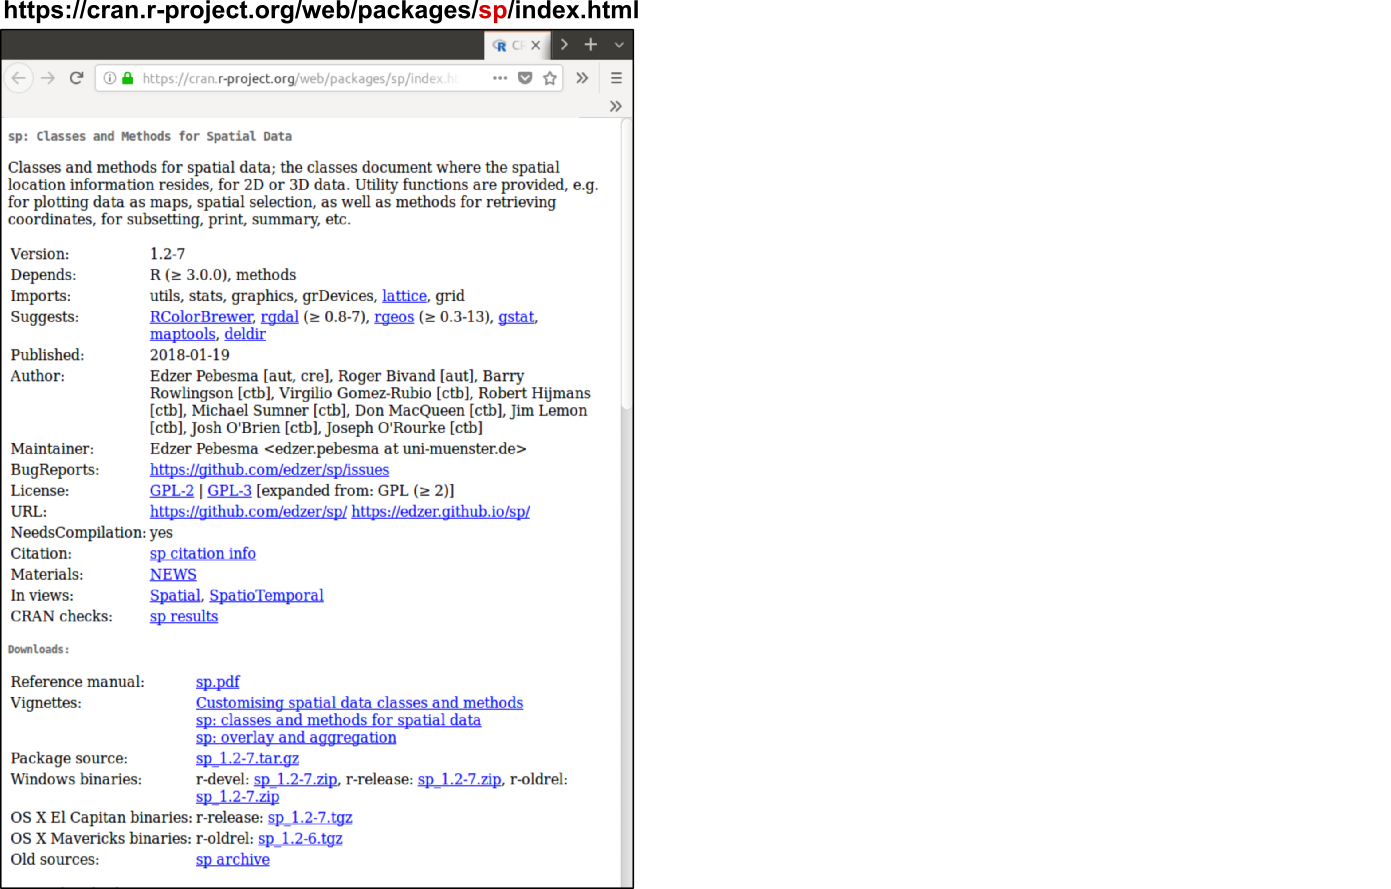
\includegraphics{imgPres/documentation_00.png}

\end{frame}

\begin{frame}{Package - Reference manual}

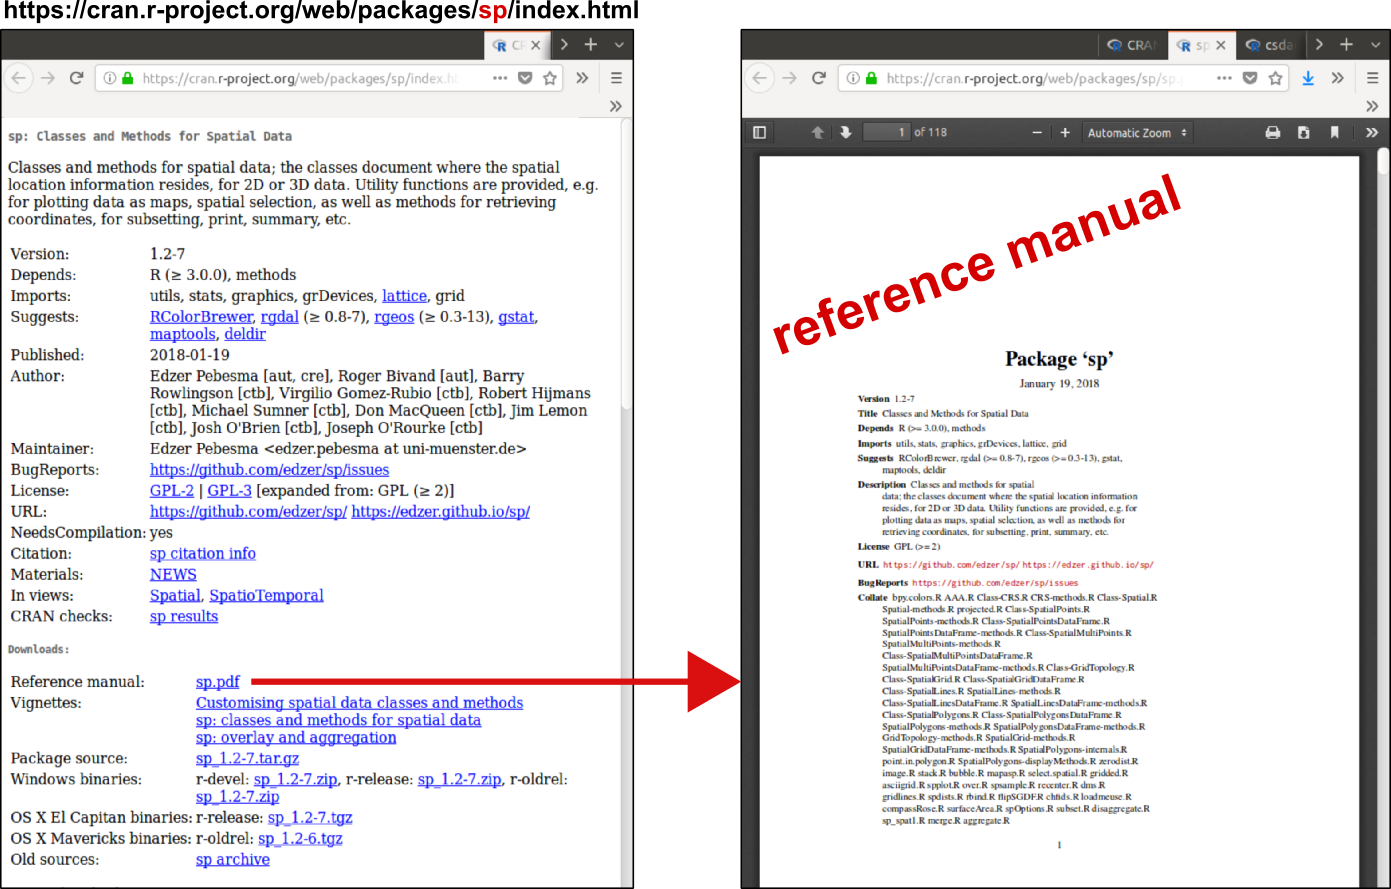
\includegraphics{imgPres/documentation_01.png}

\end{frame}

\begin{frame}{Package - Reference vignette}

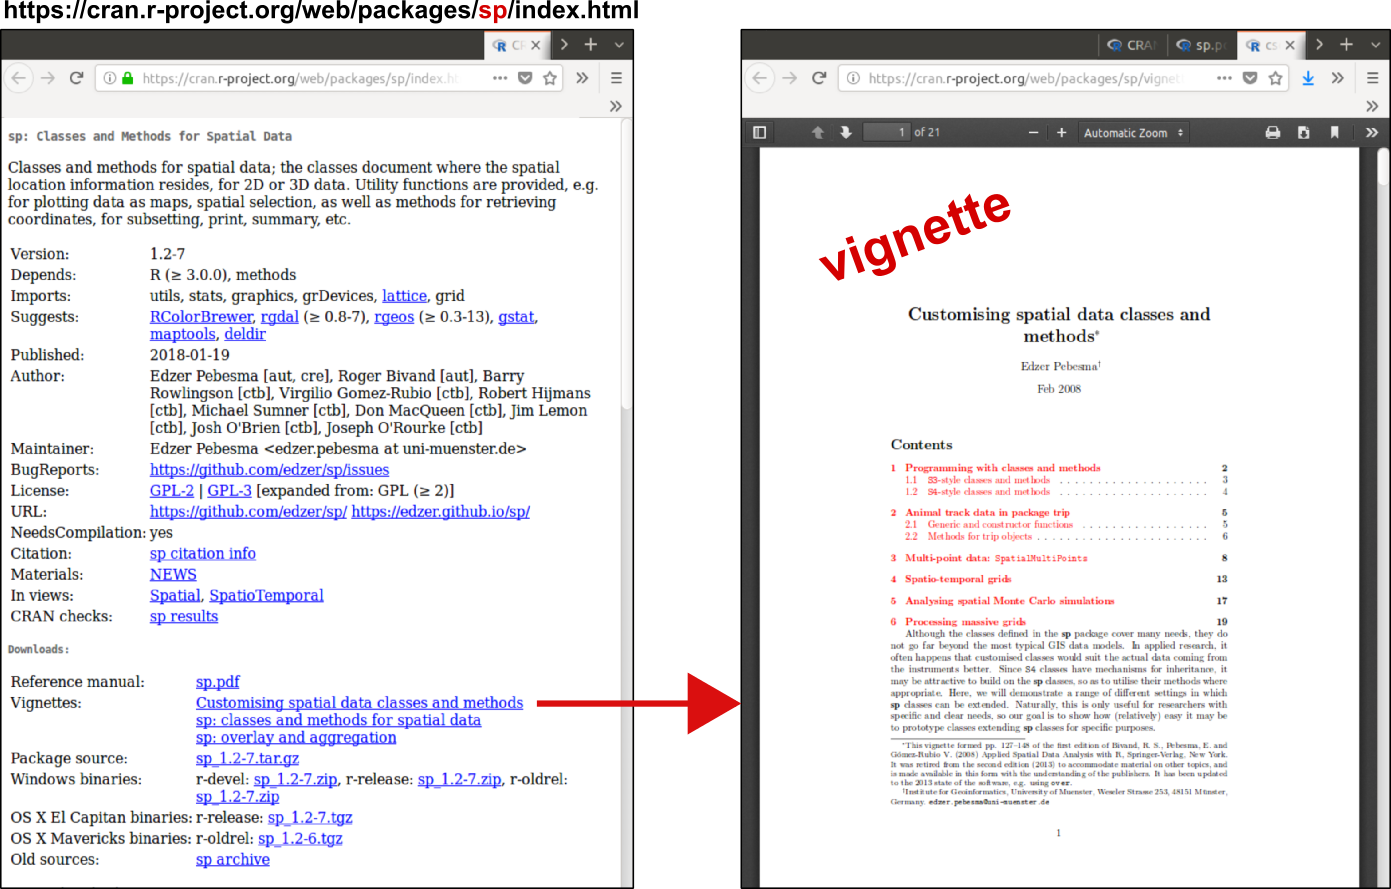
\includegraphics{imgPres/documentation_02.png}

\end{frame}

\begin{frame}{Package - Package source}

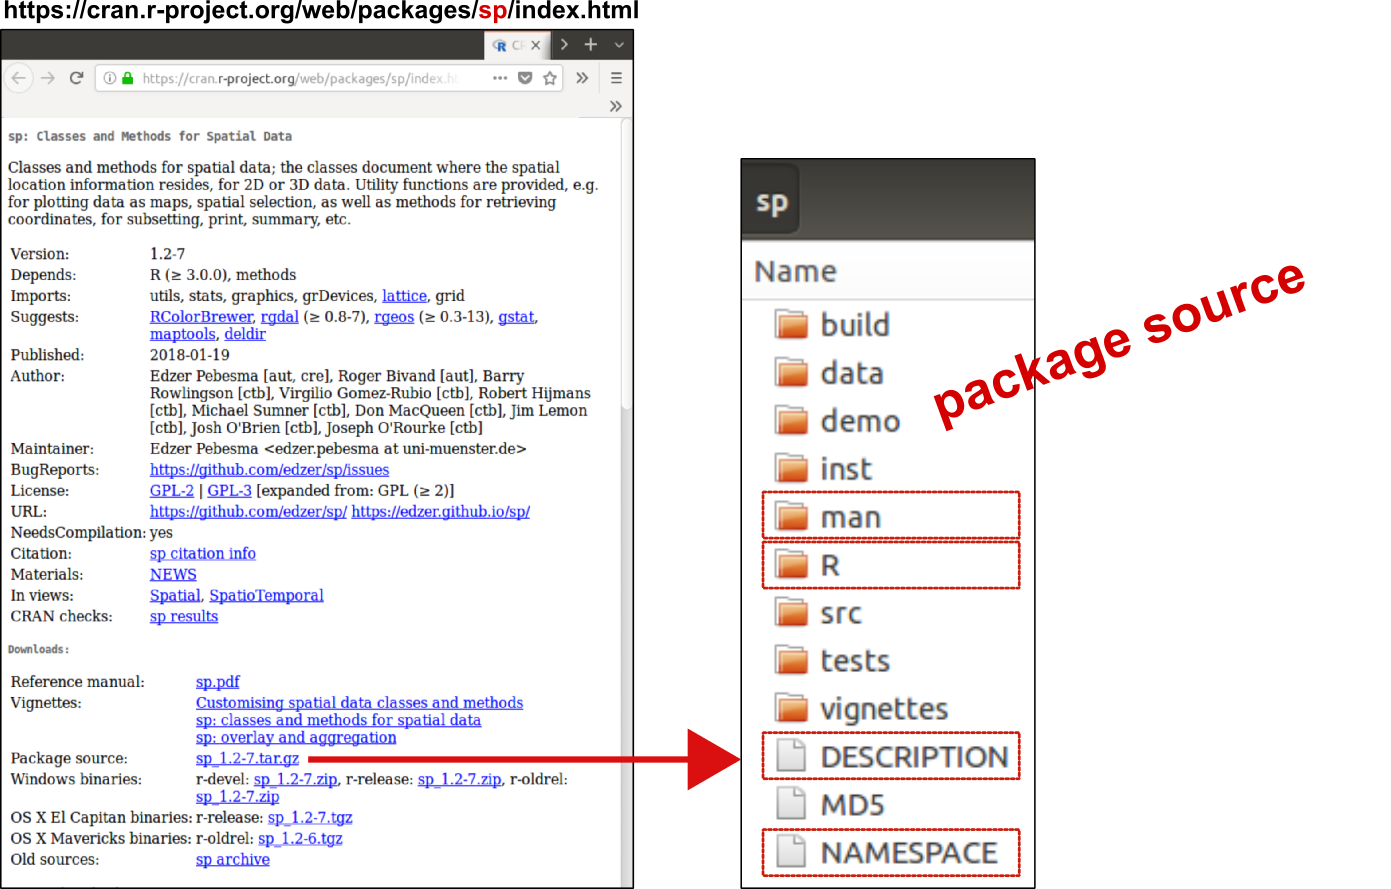
\includegraphics{imgPres/documentation_03.png}

\end{frame}

\begin{frame}{Package - Install packages hosted on CRAN}

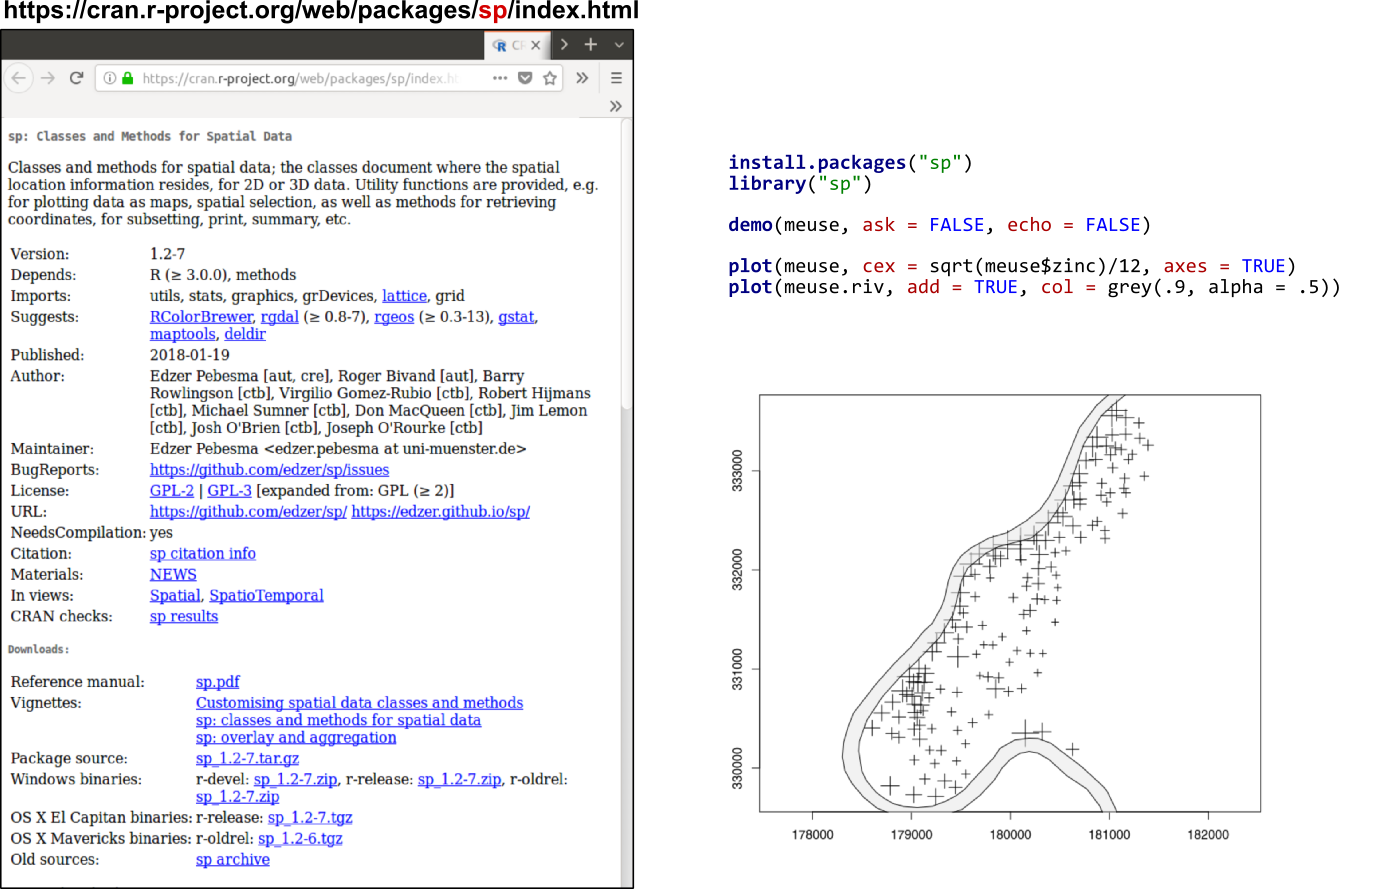
\includegraphics{imgPres/documentation_04.png}

\end{frame}

\begin{frame}[fragile]{Package - Install packages hosted on github}

\begin{Shaded}
\begin{Highlighting}[]
\NormalTok{if(!}\KeywordTok{require}\NormalTok{(}\StringTok{"devtools"}\NormalTok{)) }\KeywordTok{install.packages}\NormalTok{(}\StringTok{"devtools"}\NormalTok{)}
\NormalTok{devtools::}\KeywordTok{install_github}\NormalTok{(}\StringTok{"emanuelhuber/RGPR"}\NormalTok{)}
\end{Highlighting}
\end{Shaded}

\end{frame}

\section{Help!}\label{help}

\begin{frame}[fragile]{Getting help}

\begin{itemize}
\item
  get help on the function \texttt{plot()}:

\begin{Shaded}
\begin{Highlighting}[]
\KeywordTok{help}\NormalTok{(plot)}
\end{Highlighting}
\end{Shaded}

  or

\begin{Shaded}
\begin{Highlighting}[]
\NormalTok{?plot}
\end{Highlighting}
\end{Shaded}
\item
  get help on general terms

\begin{Shaded}
\begin{Highlighting}[]
\NormalTok{??regression}
\end{Highlighting}
\end{Shaded}
\item
  ?? \texttt{library(help\ =\ "base")} See
  \href{https://www.r-project.org/help.html}{getting help with R}
\item
  Google: ``\textbf{R Cran} how to extract rows data.frame''
\end{itemize}

\end{frame}

\section{R language}\label{r-language}

\begin{frame}[fragile]{R language}

\href{https://cran.r-project.org/doc/manuals/r-devel/R-lang.html}{Official
documentation}

\begin{block}{Main differences to MATLAB}

\begin{itemize}
\item
  \texttt{x\ \textless{}-\ x\ +\ 10} instead of \texttt{x\ =\ x\ +\ 10}
\item
  Matrices A: \texttt{A{[}1,\ 3{]}} instead of \texttt{A(1,\ 3)}
\item
  comments with \texttt{\#} instead of \texttt{\%}
\item
  no need for \texttt{;}
\item
  R is more structured: use \texttt{\{} in the loop

\begin{Shaded}
\begin{Highlighting}[]
\NormalTok{for(i in }\DecValTok{1}\NormalTok{:}\DecValTok{10}\NormalTok{)\{}
  \CommentTok{# my code here}
\NormalTok{\}}
\end{Highlighting}
\end{Shaded}

  \href{https://cran-r.c3sl.ufpr.br/doc/contrib/Hiebeler-matlabR.pdf}{Matlab
  - R}
\end{itemize}

\end{block}

\begin{block}{Exotic stuff}

\textbf{Namespace}

\texttt{packageName::functionName()}

\textbf{Pipe \texttt{\%\textgreater{}\%}}

\begin{Shaded}
\begin{Highlighting}[]
\KeywordTok{third}\NormalTok{(}\KeywordTok{second}\NormalTok{(}\KeywordTok{first}\NormalTok{(x)))}
\KeywordTok{first}\NormalTok{(x) %>%}\StringTok{ }\NormalTok{second %>%}\StringTok{ }\NormalTok{third}
\end{Highlighting}
\end{Shaded}

\href{https://bookdown.org/rdpeng/exdata/managing-data-frames-with-the-dplyr-package.html\#section}{source}

\textbf{Ellipsis \texttt{...}} fun \textless{}- function(x, \ldots{})\{
plot(x, \ldots{}) \}

\end{block}

\end{frame}

\begin{frame}[fragile]{Basic object types}

\texttt{type.of()}???

\begin{itemize}
\tightlist
\item
  numeric: \texttt{e24}, \texttt{-150.5}, \texttt{pi}
  \texttt{is.numeric()}
\item
  integer: \texttt{1L}, \texttt{-54L}, \texttt{0L} \texttt{is.integer()}
\item
  complex: ??? \texttt{is.complex()}
\item
  character: ``AUG'', ``13.12'', ``www.google.ch''
  \texttt{is.character()}
\item
  boolean (logical): \texttt{TRUE}, \texttt{FASLE} \texttt{is.logical()}
\item
  \texttt{NA}, \texttt{Inf}, \texttt{NULL}
\end{itemize}

\href{https://swcarpentry.github.io/r-novice-inflammation/13-supp-data-structures/}{check}

\end{frame}

\begin{frame}{Object classes}

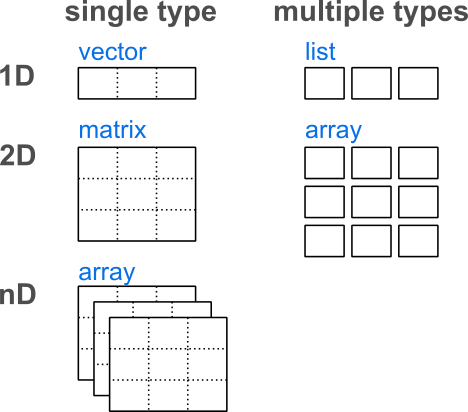
\includegraphics[width=0.45000\textwidth]{imgPres/object_types.png}

\begin{itemize}
\tightlist
\item
  numeric, matrix, list, data.frame
\item
  S3 classes: example regression
\item
  S4 classes
  \href{http://mazamascience.com/Classes/IRIS_2015/Lesson_06_WorkingWithSeismicTraces.html}{tutorial}

  \begin{itemize}
  \tightlist
  \item
    date and time
    \href{http://biostat.mc.vanderbilt.edu/wiki/pub/Main/ColeBeck/datestimes.pdf}{good
    tutorial}
  \item
    spatial data raster/sf
  \end{itemize}
\end{itemize}

\end{frame}

\begin{frame}[fragile]{Functions to understand your data}

\begin{itemize}
\tightlist
\item
  \texttt{str()}
\item
  \texttt{class()}
\item
  \texttt{unclass()}
\item
  \texttt{typeof()}
\item
  \texttt{names()} \texttt{colnames()}, \texttt{rownames()}
\item
  \texttt{dim()}, \texttt{length()}
\item
  S4: \texttt{isS4()}, \texttt{getSlots()}, \texttt{slotNames()}
\item
  attributes()
\end{itemize}

\texttt{methods(class\ =\ "sf")}

show example from ?approx

\end{frame}

\begin{frame}[fragile]{Conversion}

\begin{block}{Basic object types}

\begin{itemize}
\tightlist
\item
  \texttt{as.character()}
\item
  \texttt{as.integer()}
\item
  \texttt{as.numeric()}
\item
  \texttt{as.logical()}
\item
  \texttt{as.complex()}
\item
  \texttt{as.matrix()}
\item
  \texttt{as.data.frame()}
\item
  \texttt{as.list()}
\end{itemize}

conversion class \texttt{sf} to \texttt{sp}: as(x, ``Spatial'')

\end{block}

\end{frame}

\end{document}
